\chapter{Our Approach}
\setlength{\parindent}{0em}

\section{Overview}
We divide our work into two phases - Retargeting and Training Phase.
In Retargeting Phase we try to create a suitable motion clip for our RL agent to mimic.
In Training phase, we train our RL agent using the data obtained from the motion clip from previous phase.
\begin{figure}
\centering
  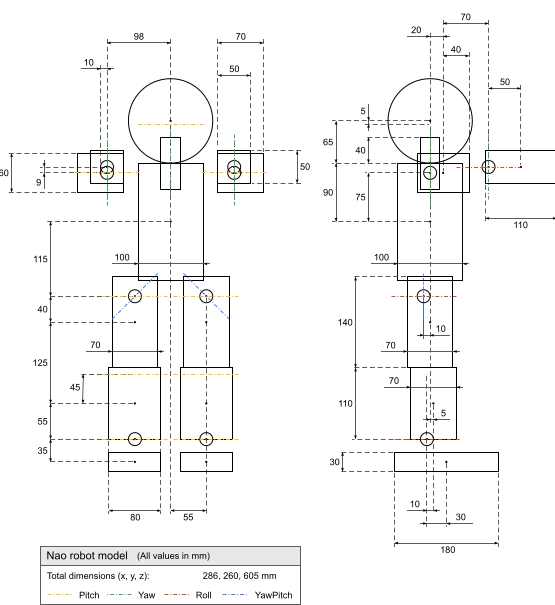
\includegraphics[width=0.7\linewidth, height=10cm,keepaspectratio]{images/nao_param.png}
  \caption{Standard Nao Agent Blueprint used in RoboCup Simulation from Simpspark specifications}
  \label{fig:nao_params}
\end{figure}

\begin{figure}
\centering
  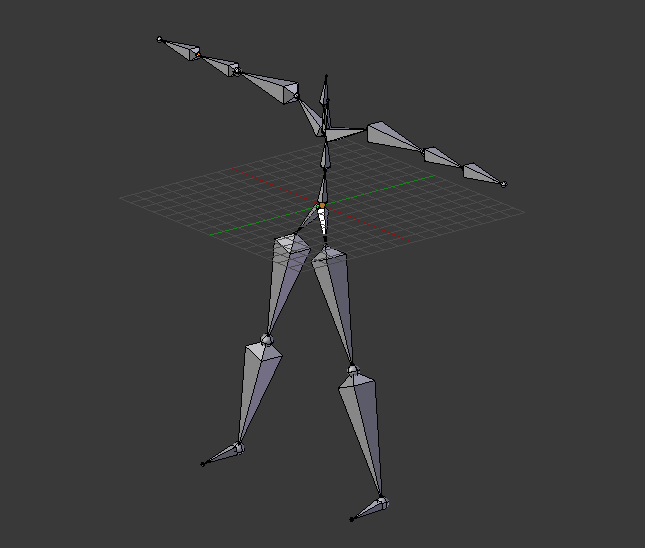
\includegraphics[width=0.7\linewidth, height=10cm,keepaspectratio]{images/mocap_hierarchy.png}
  \caption{Hierarchy of motion clip from walk in place clip before retargeting}
  \label{fig:mocap_hierarchy}
\end{figure}

\section{Retargeting Phase}
We refer to our robot's hierarchy as \texttt{nao\_hierarchy} and motion clip's bvh hierarchy as \texttt{mocap\_hierarchy}.
	


\begin{figure}[!b]
\centering
  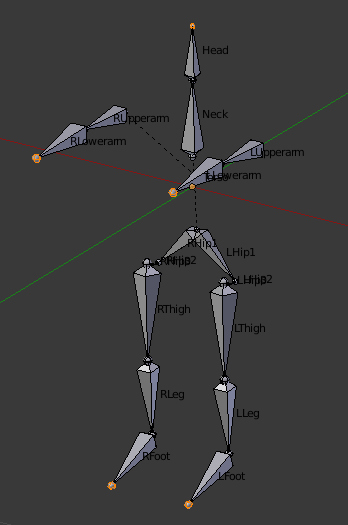
\includegraphics[width=0.7\linewidth, height=10cm,keepaspectratio]{images/nao_hierarchy.png}
  \caption{Blender view of Nao Agent Hierarchy constructed from specifications from Simspark sever and axis restrictions}
  \label{fig:nao_hierarchy}
\end{figure}

\subsection{Tools}
We chose to use Blender as our primary BVH tool due to its easier visualization and modeling interface for creating both the \texttt{nao\_hierarchy} and animation. However, some of Blender's inherent flaws in visualizing local pose orientation made it hard to debug the retargeting process. Nevertheless, due to unavailability of other BVH debugging tools, we had to use blender for most of our processing.

\subsection{Challenges}
As we can see from Fig \ref{fig:mocap_hierarchy} and Fig \ref{fig:nao_hierarchy}, both the bone lengths and number of joints are different in the \texttt{nao\_hierarchy} compared to the \texttt{mocap\_hierarchy}. Thus, to use the motion clip for our purposes we had to retarget the motion clip to our \texttt{nao\_hierarchy}. This was a non-trivial task involving unforeseen challenges. 
Firstly, Nao agent has different sets of restrictions on maximum and minimum angles at each hinge joint. Therefore, not all motions could be retargeted to \texttt{nao\_hierarchy}. Moreover, the hip joint in Nao agent has its axis aligned 45 degrees to standard axes and the complementary left and right hip joints are restricted to have same local rotations as seen in Fig \ref{fig:nao_joints}, which makes it harder to retarget any motion using any available tools online. Also, Nao agent has lesser degrees of freedom in almost all joints as compared to the \texttt{mocap\_hierarchy}. Therefore, retargeting problem for \texttt{nao\_hierarchy} was not easy to solve. Thus, to remove dependencies between the two phases, we manually crafted some easy motions like squats and hand wave for debugging training phase so that none of the retargeting errors are responsible for failure in training phase.


\subsection{Method}
We manually created a hierarchy in BVH(BioVision Hierarchical data) \cite{Maddock_motioncapture} format  for our Nao \cite{usermanual} agent (which we have referred to as \texttt{nao\_hierarchy}) using the specifications from manual as can be seen from Fig \ref{fig:nao_params}. 
\\\\
Thereafter, we gathered motion clip data from various sources like \href{http://mocap.cs.cmu.edu}{\underline{CMU}} and work of [Chris Hecker et al. 2008]\cite{sporeanim} and finally chose two simple enough clips that would be easier for agent to learn. First clip described a walk in place motion where in the agent just lifts its legs one by one trying to balance itself. Second clip was a simple hand wave motion. The motion clip originally was made for a skeleton way different than Nao's architecture as seen in Fig \ref{fig:mocap_hierarchy} (which we have referred to as \texttt{mocap\_hierarchy}).
\\\\
\begin{figure}
\centering
  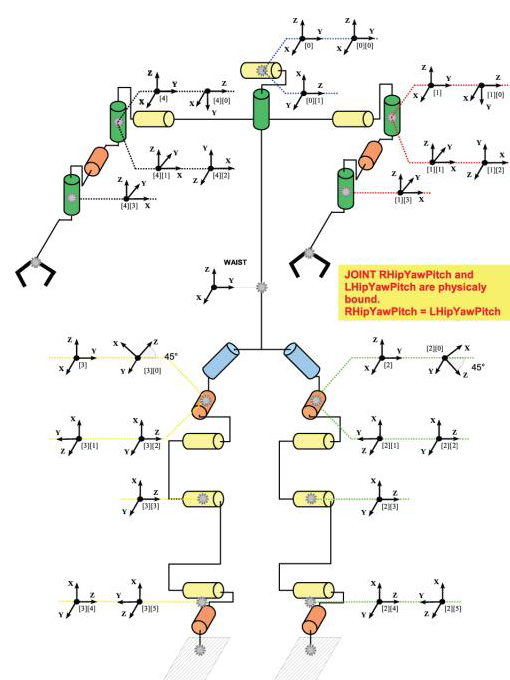
\includegraphics[width=0.7\linewidth, height=10cm,keepaspectratio]{images/nao_joints.png}
  \caption{Nao parameters indication constraints and axis alignments for all joints}
  \label{fig:nao_joints}
\end{figure}
After taking ideas from the approach of retargeting manually from [Gleicher et al. 1998]\cite{Gleicher:1998:RMN:280814.280820} we devised a mechanism to retarget any generic motion onto our \texttt{nao\_hierarchy}. This involves firstly mapping all joints in \texttt{nao\_hierarchy} to some unique joint in \texttt{mocap\_hierarchy}. Now endpoint of these joints would serve as target positions for our animation to achieve. In second step, we adjust the rest pose (where all the local joint angles are 0) and copy all rotations for every frame of motion clip from \texttt{mocap\_hierarchy} to \texttt{nao\_hierarchy}. 
Finally, we adjust global target positions of every \texttt{mocap\_hierarchy} joint for the difference in bone lengths and use standard jacobian full body inverse kinematics solver to fine tune the local rotations to make sure corresponding joints of \texttt{nao\_hierarchy} reach the respective target positions in appropriate frames. Some manual tuning was involved to make sure the final animation didn't have sudden large changes in rotations across adjacent frames.
To tackle the issue of lesser degrees of freedom in our Nao agent, we convert local retargeted rotations into Euler angles, take the required components and discard the remaining ones. This means that its possible that even though the retargeted motion looks good on unconstrained \texttt{nao\_hierarchy} but might not work after removing some specific channels. We made tweaks to rest pose and IK (Inverse Kinematics) parameters to ensure this did not happen for the motion clips we decided to retarget. 
  
\section{Training Phase} 
Now to train the agent, we resorted to policy gradient methods due to their proven advantages in domain of continuous action and state spaces. We used the renowned method of Asynchronous Advantage Actor Critic \cite{mnih2016asynchronous} to train our agent.

\subsection{States and Actions}
In our case the action space consists of the angular velocity values of 22 joints (4 on each arm, 6 in each leg, 2 for head and neck as can be seen in Fig \ref{fig:nao_joints}) of the agent. For state space, initially we just used these 22 joints' orientation in degrees, but robot was not even able to learn simple motion clips like hand waves. Applying ideas from  [Yang et al. 2017] \cite{yang2017emergence} we included various other features in our state. These include, the gyrometer values, accelerometer values, height of pelvis from the ground. For learning not to make quick movements we also had to provide input individual joint linear velocities as input to our state. Finally, to learn to periodically repeat motions, we included time as another parameter so that by only resetting time at the end of motion we can make the bot perform periodic motions. We also normalized these inputs by using empirical maximum and minimum values as seen in various simulations. Without this step, learning was very slow for some motion clips which relied on more than one kind on inputs to generate proper torques. The state space now consists of more than 50 values, as can be seen in Fig \ref{fig:neural_net}   

\subsection{Rewards}
Since our motion clips don't involve agent moving forward or any major changes in position of the robot over time, we had to worry about only two kinds of reward functions. First one is \textit{imitation reward} that makes sure that our agent mimics the motion clip to its best extent. Second one is \textit{balance reward} that is specifically purposed to make sure our agent doesn't fall down/lose balance while performing these complicated skills.

\subsubsection{Imitation Reward}
Given the current time in the simulation, we found the corresponding pose in the motion clip. By pose, we mean a tuple consisting of orientation of all 22 joints in the \texttt{nao\_hierarchy}. This pose was used to calculate a similarity metric between current state of and the desired pose in the motion clip. We experimented with various reward functions for capturing the similarity of our agent's pose and target pose of motion clip. Firstly we tried negative of the euclidean distance between the two joint orientation vectors as the similarity metric as it captures the essence of robot's deviation from its current expected pose. 
$$R_{imitation} = - \sum_{i=1}^{22} (n_i - w_i)^2$$
\texttt{where $n_i$ is the ith joint orientation in nao agent pose in degrees \\
and $w_i$ is the ith joint orientation in motion clip pose in degrees}
\vspace{1em}
\\
This wasn't working very well with the A3C algorithm as the learning curve suddenly dropped after 20-30k iterations leading to poorly trained model. After further experiments we found another function of the euclidean distance to stabilize the learning process. 
$$R_{imitation} = e^{- \sum_{i=1}^{22} (n_i - w_i)^2}$$
\texttt{where $n_i$ is the ith joint orientation in nao agent pose in degrees \\
and $w_i$ is the ith joint orientation in motion clip pose in degrees} 
\subsubsection{Balancing Reward}
We experimented with various strategies for this reward too. One way we tried was to check if the agent is about to fall or is already down. This involved tuning falling condition threshold by using accelerometer data from the agent. We then terminated the episode with large negative reward whenever this happened.  \\

$$R_{balance} =
    \begin{cases*}
      -k & if \ \ agent fallen \\ 
       \ 0  & otherwise
    \end{cases*}
$$
\texttt{where $k$ is a large positive constant}
\vspace{1em}
\\
This was not working well due to the fact that agent learnt to "almost" fall at the end of motion clip losing stability way too soon getting overall high rewards. So, to make sure agent never ever loses stability we used  a reward corresponding to maintaining pelvis height from ground above certain level and keeping gyrometer values below some empirical threshold. Using this reward we found that agent doesn't learn to fall but tries to maintain stability throughout the simulation.
$$R_{balance1} =
    \begin{cases*}
        k1 & if \ \ |gyr| < t1 \\ 
       \ 0  & otherwise
    \end{cases*}
$$
$$R_{balance2} =
    \begin{cases*}
        e^{\frac{1}{h}} & if \ \ h > t2 \\ 
       \ 0  & otherwise
    \end{cases*}
$$
\texttt{where $k1$ is a small positive reward in case the gyrometer values ($gyr$) are less than a threshold ($t1$)\\
and  $h$ is the height of pelvis from the ground \\
and $t2$ is another threshold for the height}
\\\\
Finally the total reward at the end of one action step is as following

$$R_{total} = a \times R_{imitiation} + b \times R_{balance1} + c \times R_{balance2}$$
\texttt{where $a,b,c$ are weights tuned empirically for each of the three different rewards)}
\vspace{1em}
\\
\begin{figure}
\centering
  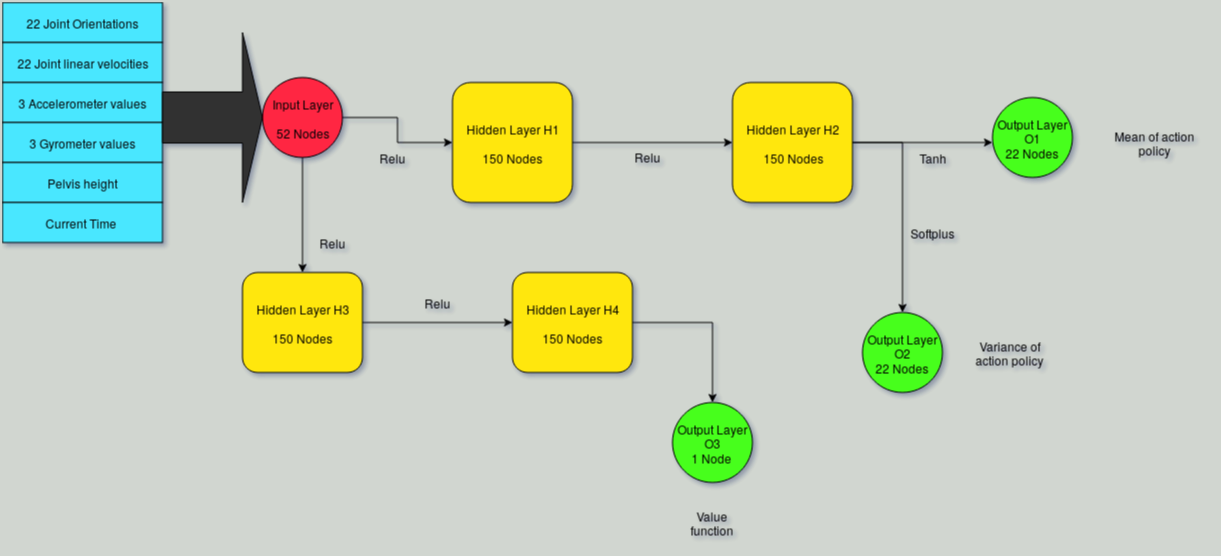
\includegraphics[width=1\linewidth, height=15cm,keepaspectratio]{images/neural_net.png}
  \caption{Neural Network architecture for design used to train robot via A3C.}
  \label{fig:neural_net}
\end{figure}

\subsection{Neural Net}
As with other parameters of this phase we experimented with various architectures for neural network. Finally, we settled for an architecture where policy was modeled by two neural networks sharing two hidden layers to model mean and variance of policy (actor network). We used an independent additional network for computing value function (critic network). The two hidden layers enable the robot to learn even complex actions for every joint. 
The number of nodes in hidden network was experimented with, and we found that since the state space is large, models trained with around 150 nodes in each hidden layer are good enough to mimic the motions to great accuracies. Also, this kept a balance between time to learn and level of skill learnt.
\\\\
For mean of the policy, we tried training both with and without tanh activation at the output layer(can be seen in Fig \ref{fig:neural_net}). Since some motions might need larger angular velocities than the unit value from tanh's output, we had to scale the means by a span threshold. When threshold was kept small, the agent learnt to alternate between extreme ends just to make sure to follow the motion clip. This created undesired vibrations in final trained model. Therefore, we tuned the threshold to stop such oscillating behavior of our agent. Without the tanh activation, in some cases where the means values went very high, they didn't return to their stable values (due to unpredictable behavior in other robot joints at high angular velocities). Thus, we settled on using tanh as the activation at the output layer for mean. For variance to make it positive we used a standard softplus activation. Regarding inner layer activations, we found that neither sigmoid nor tanh activations gave good results perhaps due to dampened gradients and slow overall learning. Relu activations proved to be best amongst all others and made it to the final architecture.